%%%%%%%%%%%%%%%%%%%%%%%%%%%%%%%%%%%%%%%%%%%
% File      : res
% Author    : th202608@pleiades068.intra.cea.fr
% Date      : 15 oct. 2012
% Directory : /home/th202608/codes/tfel/tests/Broyden/
%%%%%%%%%%%%%%%%%%%%%%%%%%%%%%%%%%%%%%%%%%%

\documentclass[12pt]{article}

\usepackage[utf8]{inputenc}

\usepackage[dvips]{graphicx}
\usepackage[dvips]{hyperref}

\usepackage{mathematiques}
\usepackage{mecanique}
\usepackage{couleurs}
\usepackage{presentation}
\usepackage{array}

\usepackage[frenchb]{babel}

\newcommand{\pleiades}{\texttt{pleiades}}
\newcommand{\mfront}{\texttt{mfront}}
\newcommand{\cyrano}{\texttt{cyrano}}
\newcommand{\castem}{\texttt{Cast3M}}
\newcommand{\pycastem}{\texttt{pyCast3M}}
\newcommand{\umat}{\texttt{umat}}
\newcommand{\sirius}{\texttt{sirius}}

\newcommand{\nbzrc}{$NbZrC$}
\newcommand{\upuc}{$\paren{U,Pu}C$}
\newcommand{\sic}{$SiC$}

\newcommand{\windows}{\href{http://www.microsoft.com/france/windows/default.mspx}{\texttt{Windows}}}
\newcommand{\linux}{\href{http://www.kernel.org/}{\texttt{linux}}}
\newcommand{\excel}{\href{http://www.microsoft.com/france/office/2007/programs/excel/overview.mspx}{\texttt{Microsoft Office Excel}}}

\newcommand{\code}[1]{
  \psframebox[linecolor=ceaorange,shadow=true,blur=true]{
    \begin{minipage}[htbp]{1.0\linewidth}
      \ttfamily\scriptsize #1
    \end{minipage}
  }
}

\begin{document}

\section{Introduction}

\paragraph{Utilisation de \mfront{} dans \cyrano{}}

Un effort de développement a été fait pour faciliter l'introduction
d'une loi de comportement mécanique dans \cyrano{} en utilisant le
formalisme de appels externes utilisé par \mfront{}\footnote{Il s'agit
d'une modification de l'interface \umat{} que nous avons proposé pour
permettre l'appel de lois de comportement mécanique dans des
bibliothèques externes. Auparavant une recompilation partielle de
\castem{} était nécessaire pour ajouter une loi. Outre la relative
complexité de cette recompilation pour un utilisateur final, cette façon
de procéder était incompatible avec l'utilisation faite de \castem{} par
les applications \pleiades{} via l'interface
\pycastem~\cite{t.06:_implan}.}.

\paragraph{Utilisation de \mfront{} au DER/SESI}

\section{Propriétés matériaux}

Les propriétés matériau sont l'un des éléments de connaissance
essentiel des matériaux. Elles sont également le plus simple à
traiter, ce qui a naturellement conduit à les regrouper au sein de
base de données, notamment la base de données \sirius{}.

\subsection{Généralités}

Une propriété matériau est supposée dépendre de manière univoque des
valeurs actuelles d'un ensemble de variables d'état thermodynamique du
matériau. Ainsi, définir une propriété matériau revient à donner la
liste de ces variables d'état et la relation fonctionnelle qui permet
de la calculer, cette relation fonctionnelle étant souvent une
corrélation basée sur des mesures expérimentales.

\paragraph{Bornes} Les variables d'états peuvent posséder des bornes
intrinsèques~: une température ne peut être négative, une porosité
supérieure à \(1\). Ces bornes intrinsèques sont dénommées dans la
suite \og~bornes physiques~\fg. Par ailleurs, la corrélation définissant
la propriété matériau a souvent été établie sur certain domaine~:
les limites de ce domaine expérimental seront dénommées
\og~bornes de validité~\fg (de la corrélation). 

\subsection{Interfaces disponibles} Les interfaces disponibles pour cet analyseur
sont~:
\begin{itemize}
\item l'interface \texttt{c} pour une utilisation dans des codes écrits
  dans ce language~;
\item l'interface \texttt{fortran} pour une utilisation dans des codes
  écrits dans ce language~;
\item l'interface \texttt{c++} pour une utilisation dans des codes écrits
  dans ce language. Cette interface est actuellement utilisée par la
  partie physico-chimique de \texttt{Germinal v2}~;
\item l'interface \texttt{castem} pour une utilisation dans le code aux
  éléments finis \castem{}. L'utilisation de cette interface a été
  décrite ailleurs~\cite{helfer07:_utilis} et nécessite une version
  modifiée de \castem{}. Les modifications en question ont été
  proposées pour une intégration dans la version officielle de
  \castem{}~;
\item l'interface \texttt{python} pour une utilisation dans des codes écrits
  dans ce language~;
\item l'interface \texttt{octave} pour une utilisation dans des codes écrits
  dans ce language~;
\item l'interface \texttt{gnuplot} pour une visualisation des courbes d'évolution
  des propriétés matériau en fonction de leur paramètres~;
\item l'interface \texttt{pleiades} pour une utilisation dans les applications
  de cette plateforme \pleiades{}~;
\end{itemize}

\begin{table}[htbp]
  \centering
  \begin{tabular}[htbp]{|l|l|l|}
    \cline{2-3}
    \multicolumn{1}{c|}{\mbox{}} & \multicolumn{2}{c|}{Nom de la bibliothèque générée} \\
    \hline
    Interface & sous \windows{} & sous \linux{} \\
    \hline
    \hline
    \texttt{c}        & libMaterialLaw.dll       & libMaterialLaw.so    \\
    \hline
    \texttt{c++}      & libCppMaterialLaw.dll    & libCppMaterialLaw.so \\
    \hline
    \texttt{castem}   & libCastemMaterialLaw.dll & libCastemMaterialLaw.so \\
    \hline
    \texttt{python}   & materiallaw.dll & materiallaw.so\\
    \hline
    \texttt{pleiades} & libPleiadesMaterialLaw.dll 
                      & libPleiadesMaterialLaw.so   \\
    \hline
  \end{tabular}
  \caption{Nom par défaut de la bibliothèque générée en
    fonction de l'interface choisie.}
  \label{tab:biblio_vs_interface}
\end{table}

\paragraph{Bibliothèques générés} Chacune des interfaces \texttt{c},
\texttt{c++}, \texttt{castem}, \texttt{python} ou \texttt{pleiades} va
générer une bibliothèque de fonction dont le nom par défaut est donné au
tableau~\ref{tab:biblio_vs_interface}. Ce nom peut être modifié par
le mot clé {\tt @Material} ou le mot clé {\tt @Library}.

\paragraph{Autres utilisations} Bien que ces interfaces aient été
construites pour une utilisation particulière, il est possible
d'utiliser les bibliothèques générées dans des contextes
distincts. Ainsi, le paragraphe \ref{sec:inter-avec-excel} montre
comment l'interface \castem{} peut être utilisée pour interagir avec
\excel{}.

\subsection{Exemple du module d'\nom{Young} du \sic{}}
\label{sec:module-dnomyoung-du}

\nom{Snead} a proposée une corrélation donnant le module d'\nom{Young} 
du \sic{} en fonction de la température et de la porosité 
sous la forme~:
\begin{equation}
  \label{eq:youngmodulussnead}
  E\paren{T,p} = \paren{E_{0}-B\,T\,\exp\paren{-\Frac{T_{0}}{T}}}\exp\paren{-C\,p}
\end{equation}
où~:
\begin{minipage}[t]{0.75\linewidth}
  \begin{itemize}
  \item \(T\) est la température~;
  \item \(p\) est la porosité~;
  \item \(E_{0}\), \(B\), \(T_{0}\) \(C\) sont des coefficients.
  \end{itemize}
\end{minipage}

\begin{figure}[htbp]
  \centering
  \code{{\ttfamily \noindent
\ttfamily
\hlstd{@Parser MaterialLaw}\hlsym{;}\hspace*{\fill}\\
\hlstd{@Law}\hlstd{\ \ \ \ }\hlstd{SIC\textunderscore YOUNGMODULUS\textunderscore SNEAD}\hlsym{;}\hspace*{\fill}\\
\hlstd{@Author Thomas Helfer}\hlsym{;}\hspace*{\fill}\\
\hlstd{@Date}\hlstd{\ \ \ }\hlstd{}\hlnum{2007}\hlstd{}\hlsym{{-}}\hlstd{}\hlnum{12}\hlstd{}\hlsym{{-}}\hlstd{}\hlnum{06}\hlstd{}\hlsym{;}\hspace*{\fill}\\
\hlstd{\hspace*{\fill}\\
@Description}\hlsym{\{}\hspace*{\fill}\\
\hlstd{}\hlstd{\ \ }\hlstd{Journal of Nuclear Materials }\hlkwd{371 }\hlstd{}\hlsym{( }\hlstd{}\hlnum{2007 }\hlstd{}\hlsym{) }\hlstd{}\hlnum{329}\hlstd{}\hlsym{{-}}\hlstd{}\hlnum{377}\hspace*{\fill}\\
\hlstd{}\hlstd{\ \ }\hlstd{Handbook of SiC properties }\hlkwa{for }\hlstd{fuel performance modeling\hspace*{\fill}\\
}\hlstd{\ \ }\hlstd{L}\hlsym{.}\hlstd{L}\hlsym{. }\hlstd{SNEAD et al}\hlsym{.}\hspace*{\fill}\\
\hlstd{}\hlstd{\ \ }\hlstd{Pages }\hlnum{339 }\hlstd{et }\hlnum{340 }\hlstd{}\hlsym{{-} }\hlstd{é}\hlkwd{quations }\hlstd{}\hlsym{(}\hlstd{}\hlnum{17}\hlstd{}\hlsym{) }\hlstd{}\hlkwd{et }\hlstd{}\hlsym{(}\hlstd{}\hlnum{18}\hlstd{}\hlsym{)}\hspace*{\fill}\\
\hlstd{}\hlsym{\}}\hspace*{\fill}\\
\hlstd{}\hspace*{\fill}\\
\hlslc{// changing the name of output}\hspace*{\fill}\\
\hlstd{@Output E}\hlsym{;}\hspace*{\fill}\\
\hlstd{}\hspace*{\fill}\\
\hlslc{// input of the law}\hspace*{\fill}\\
\hlstd{@Input T}\hlsym{,}\hlstd{p}\hlsym{;}\hspace*{\fill}\\
\hlstd{}\hspace*{\fill}\\
\hlslc{// variables bounds}\hspace*{\fill}\\
\hlstd{@PhysicalBounds T in }\hlsym{{[}}\hlstd{}\hlnum{0}\hlstd{}\hlsym{:{*}{[};}\hspace*{\fill}\\
\hlstd{@PhysicalBounds p in }\hlsym{{[}}\hlstd{}\hlnum{0}\hlstd{}\hlsym{:}\hlstd{}\hlnum{1}\hlstd{}\hlsym{{]};}\hspace*{\fill}\\
\hlstd{\hspace*{\fill}\\
@Function}\hlsym{\{}\hspace*{\fill}\\
\hlstd{}\hlstd{\ \ }\hlstd{}\hlkwb{const real }\hlstd{E0 }\hlsym{=}\hlstd{\ \ }\hlsym{}\hlstd{}\hlnum{460.00}\hlstd{E9 }\hlsym{;}\hspace*{\fill}\\
\hlstd{}\hlstd{\ \ }\hlstd{}\hlkwb{const real }\hlstd{B}\hlstd{\ \ }\hlstd{}\hlsym{=}\hlstd{\ \ \ \ }\hlsym{}\hlstd{}\hlnum{0.04}\hlstd{E9 }\hlsym{;}\hspace*{\fill}\\
\hlstd{}\hlstd{\ \ }\hlstd{}\hlkwb{const real }\hlstd{T0 }\hlsym{=}\hlstd{\ \ }\hlsym{}\hlstd{}\hlnum{962.00}\hlstd{\ \ \ }\hlnum{}\hlstd{}\hlsym{;}\hspace*{\fill}\\
\hlstd{}\hlstd{\ \ }\hlstd{}\hlkwb{const real }\hlstd{C}\hlstd{\ \ }\hlstd{}\hlsym{=}\hlstd{\ \ \ \ }\hlsym{}\hlstd{}\hlnum{3.57}\hlstd{\ \ \ }\hlnum{}\hlstd{}\hlsym{;}\hspace*{\fill}\\
\hlstd{}\hlstd{\ \ }\hlstd{E }\hlsym{= (}\hlstd{E0}\hlsym{{-}(}\hlstd{B}\hlsym{{*}}\hlstd{T}\hlsym{{*}}\hlstd{}\hlkwd{exp}\hlstd{}\hlsym{({-}}\hlstd{T0}\hlsym{/}\hlstd{T}\hlsym{))){*}}\hlstd{}\hlkwd{exp}\hlstd{}\hlsym{({-}}\hlstd{C}\hlsym{{*}}\hlstd{p}\hlsym{);}\hspace*{\fill}\\
\hlstd{}\hlsym{\} }\hlstd{}\hlslc{// end of function}\hlstd{}\hspace*{\fill}\\
\mbox{}
\normalfont
}}  
  \caption{Implantation du module d'\nom{Young} du \sic{} en \mfront{}.}
  \label{fig:mfront_sic_youngmodulus}
\end{figure}

La figure~\ref{fig:mfront_sic_youngmodulus} donne le code source
implémentant cette corrélation.

\paragraph{Le mot clé \texttt{@Parser}} La première ligne, commençant
par le mot clé \texttt{@Parser}, décrit le type d'analyseur utilisé,
ici \texttt{MaterialLaw}.

\paragraph{Le mot clé \texttt{@Law}} La second ligne, commençant par
le mot clé \texttt{@Law}, donne le nom de la propriété matériau. Ce
nom sera utilisé pour l'appel à la propriété matériau (nom de la
fonction ou de la classe générée suivant l'interface utilisée).

\paragraph{Le mot clé \texttt{@Material}}  Le mot clé \texttt{@Material},
non utilisé ici, sert à regrouper plusieurs propriétés d'un même
matériau dans une même bibliothèque.

\paragraph{Les mots clé \texttt{@Author} et \texttt{@Date}} La
troisième et la quatrième ligne renseignent respectivement l'auteur du
fichier et la date de création à l'aide des mots clés \texttt{@Author}
et \texttt{@Date}.

\paragraph{Le mot clé \texttt{@Description}} Le mot clé
\texttt{@Description} permet de donner les références bibliographiques
d'où la corrélation est extraite ou tout commentaire sur son origine.

\paragraph{Le mot clé \texttt{@Output}} Le mot clé \texttt{@Output}
change le nom de la propriété matériau calculée. Par défaut, celle-ci
s'appelle \texttt{res}.

\paragraph{Le mot clé \texttt{@Input}} Le mot clé \texttt{@Input}
donne la liste des variables d'état dont dépend la propriété. Les
variables peuvent être déclarées en une fois ou par plusieurs
utilisations consécutives du mot clé \texttt{@Input}. L'ordre de
déclaration des variables peut être important suivant l'interface
utilisé~: ainsi la fonction générée par les interface \texttt{c} ou
\texttt{castem} prendront leur arguments dans l'ordre de déclaration
utilisé dans le fichier \mfront{}.

\paragraph{La méthode \texttt{setGlossaryName}} La méthode
\texttt{setGlossaryName}, non utilisée ici, permet de préciser le nom
du champ associé à la variable dans \pleiades{}.

\paragraph{Le mot clé \texttt{@PhysicalBounds}} Le mot clé
\texttt{@PhysicalBounds} définit les bornes physiques des variables
d'état définies plus haut. Ici nous indiquons qu'une température ne
peut être négative et qu'une porosité est comprise entre \(0\) et
\(1\). Les cas de dépassement de ces bornes sont très souvent liées à
des problèmes graves des codes (erreur de programmation, solutions
inacceptables). Pour ces raisons, la plupart des interfaces
signaleront une erreur au code appelant, conduisant généralement à son
arrêt.

\paragraph{Le mot clé \texttt{@Bounds}} Le mot clé \texttt{@Bounds},
non utilisé ici, définit les bornes de validité de la corrélation. Les
cas de dépassement de ces bornes peuvent être d'origine diverse, et
peuvent parfois être acceptable.  La plupart des interface permettent
de paramétrer leur réaction en cas de dépassement des bornes de
validité. Trois politiques sont généralement retenues~:
\begin{itemize}
\item \texttt{STRICT}, qui conduit à signaler une erreur au code
appelant~;
\item \texttt{WARNING}, qui conduit à afficher un message
d'avertissement sans génération d'erreur~;
\item \texttt{NONE}, qui ignore le dépassement~;
\end{itemize} Par défaut, la politique \texttt{NONE} est utilisée. La
manière de déclarer ces politiques dépend de l'interface~:
\begin{itemize}
\item l'interface {\texttt{c++}} lit la valeur de variable
d'environnement \texttt{OUT\_\-OF\_\-BOUND\_\-POLICY}~;
\item l'interface {\texttt{castem}} lit la valeur de variable
d'environnement \texttt{CASTEM\_\-OUT\_\-OF\_\-BOUND\_\-POLICY}~;
\item l'interface {\texttt{python}} lit la valeur de variable
d'environnement \texttt{PYTHON\_\-OUT\_\-OF\_\-BOUND\_\-POLICY}~;
\item l'interface {\texttt{octave}} lit la valeur de variable globale
\texttt{OCTAVE\_\-OUT\_\-OF\_\-BOUND\_\-POLICY}~;
\item l'interface {\texttt{pleiades}} dépend de la valeur de la
variable de type \texttt{String} \texttt{OutOfBoundsPolicy} qui doit
être définie dans le fichier d'entrée.
\end{itemize}

\paragraph{Le mot clé \texttt{@Function}} Le mot clé
\texttt{@Function} permet de définir le code (en \texttt{c++}) utilisé
pour définir la propriété matériau. Le fait que le code soit en fait
du \texttt{c++} est ici anecdotique tant le code est proche de
l'équation~\eqref{eq:youngmodulussnead}.

\subsection{Interaction avec \excel{}}
\label{sec:inter-avec-excel}

% \excel{} apparaît comme un logiciel particulièrement apprécié par les
% utilisateurs \celaeno{}. Nous montrons ici que \mfront{} permet
% simplement d'interagir avec lui. 

\paragraph{De \mfront{} à \excel{}}
En premier lieu, les librairies de propriétés matériau
générées par \mfront{} avec l'interface \castem{} peuvent être directement
appelées depuis \excel{}. 

\begin{figure}[htbp]
  \centering
  \code{
    \noindent
\ttfamily
\hlstd{}\hlkwa{Declare Function }\hlstd{SIC\textunderscore YOUNGMODULUS\textunderscore SNEAD }\hlkwa{Lib }\hlstd{}\hlstr{"libCastemMaterialLaw"}\hlstd{ }\hlsym{(}\hlstd{temp }\hlkwa{As }\hlstd{}\hlkwb{Double}\hlstd{}\hlsym{) }\hlstd{}\hlkwa{As }\hlstd{}\hlkwb{Double}\hspace*{\fill}\\
\hlstd{}\hspace*{\fill}\\
\hlkwa{Public Function }\hlstd{}\hlkwd{LoiMat}\hlstd{}\hlsym{(}\hlstd{ParamArray }\hlkwd{VarTableau}\hlstd{}\hlsym{())}\hspace*{\fill}\\
\hlstd{}\hlstd{\ \ \ \ }\hlstd{}\hlkwa{Dim }\hlstd{}\hlkwd{v}\hlstd{}\hlsym{(}\hlstd{}\hlnum{2}\hlstd{}\hlsym{) }\hlstd{}\hlkwa{As }\hlstd{}\hlkwb{Double}\hspace*{\fill}\\
\hlstd{}\hlstd{\ \ \ \ }\hlstd{}\hlkwd{v}\hlstd{}\hlsym{(}\hlstd{}\hlnum{0}\hlstd{}\hlsym{) = }\hlstd{}\hlkwd{VarTableau}\hlstd{}\hlsym{(}\hlstd{}\hlnum{0}\hlstd{}\hlsym{)}\hspace*{\fill}\\
\hlstd{}\hlstd{\ \ \ \ }\hlstd{}\hlkwd{v}\hlstd{}\hlsym{(}\hlstd{}\hlnum{1}\hlstd{}\hlsym{) = }\hlstd{}\hlkwd{VarTableau}\hlstd{}\hlsym{(}\hlstd{}\hlnum{1}\hlstd{}\hlsym{)}\hspace*{\fill}\\
\hlstd{}\hlstd{\ \ \ \ }\hlstd{LoiMat }\hlsym{= }\hlstd{}\hlkwd{SIC\textunderscore YOUNGMODULUS\textunderscore SNEAD}\hlstd{}\hlsym{(}\hlstd{}\hlkwd{v}\hlstd{}\hlsym{(}\hlstd{}\hlnum{0}\hlstd{}\hlsym{))}\hspace*{\fill}\\
\hlstd{}\hlkwa{End Function}
  }
  \caption{Appel d'une loi externe depuis \excel{}.}
  \label{fig:excelvba}
\end{figure}

La figure~\ref{fig:excelvba} représente une macro
\texttt{Visual Basic} permettant cet appel. Elle déclare une fonction
\texttt{LoiMat} qui peut être directement utilisée dans un classeur
sous la forme~:
\begin{center}
  \begin{minipage}[htbp]{0.9\linewidth}
    \small
    \texttt{=LoiMat(\$A\$1,A3)}
  \end{minipage}
\end{center}
qui calculera dans cet exemple le module d'\nom{Young} du \sic{} en
fonction de la valeur de la température, lue dans la cellule
\texttt{\$A\$1} et de la valeur de la porosité, lue dans la cellule
\texttt{A3}. 

Le passage par la macro \texttt{Visual Basic} décrite en
figure~\ref{fig:excelvba} est assez lourd et nous pensons être en
mesure de nous en passer prochainement, rendant encore plus simple
l'utilisation des librairies matériau issue de \mfront{} dans
\excel{}.

\begin{figure}[htbp]
  \centering
  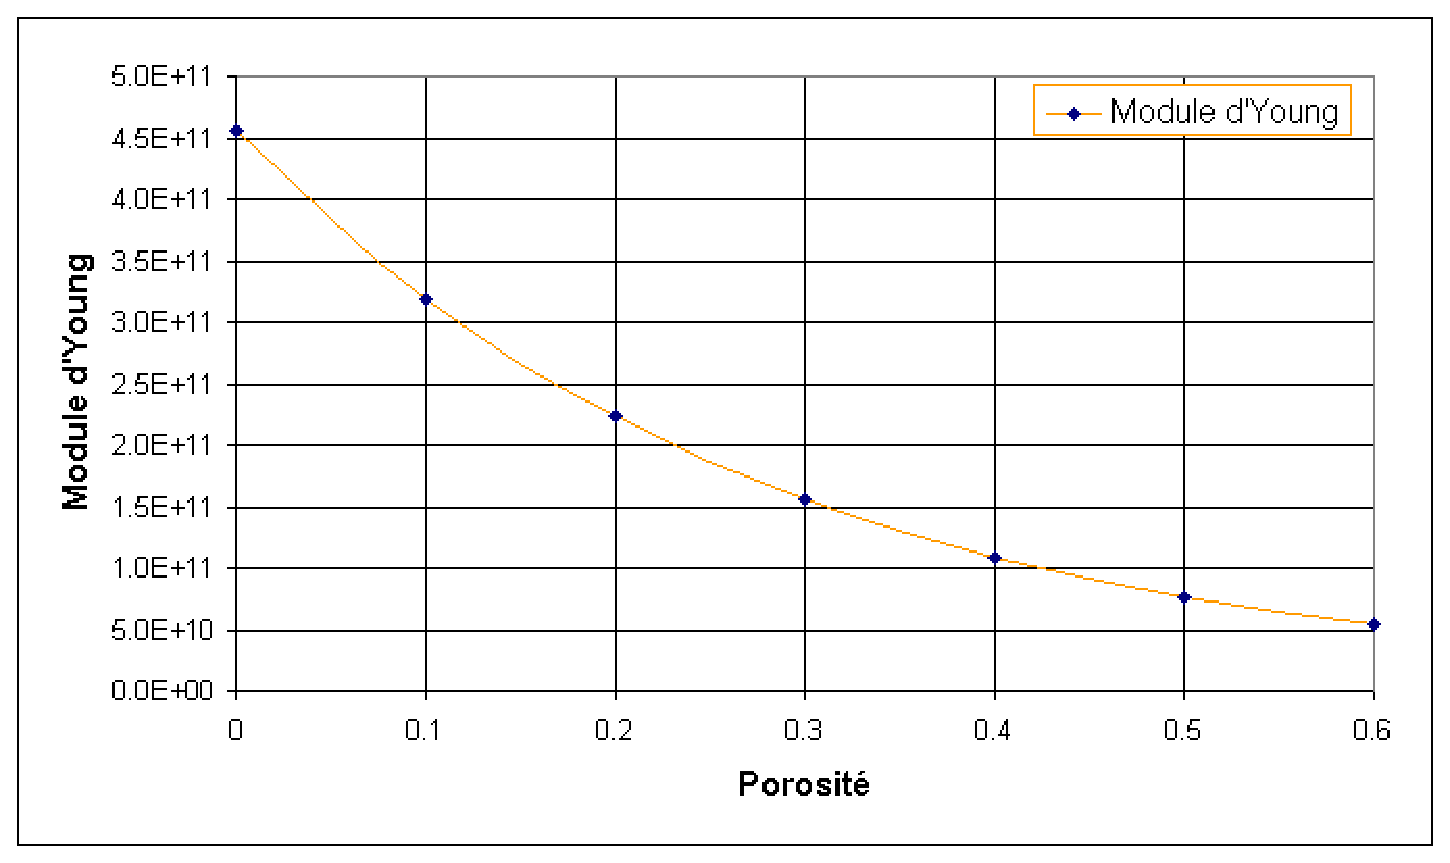
\includegraphics[width=9cm]{Images/mfrontexcel.eps}
  \caption{Graphique \excel{} réalisé à partir d'une
    bibliothèque dynamique généré par \mfront{}.}
  \label{fig:mfrontexcel}
\end{figure}

La figure~\ref{fig:mfrontexcel} montre la dépendance du module
d'\nom{Young} du \sic{} en fonction de la porosité en se basant
sur l'exemple traité au paragraphe~\ref{sec:module-dnomyoung-du}.

\begin{figure}[htbp]
  \centering
  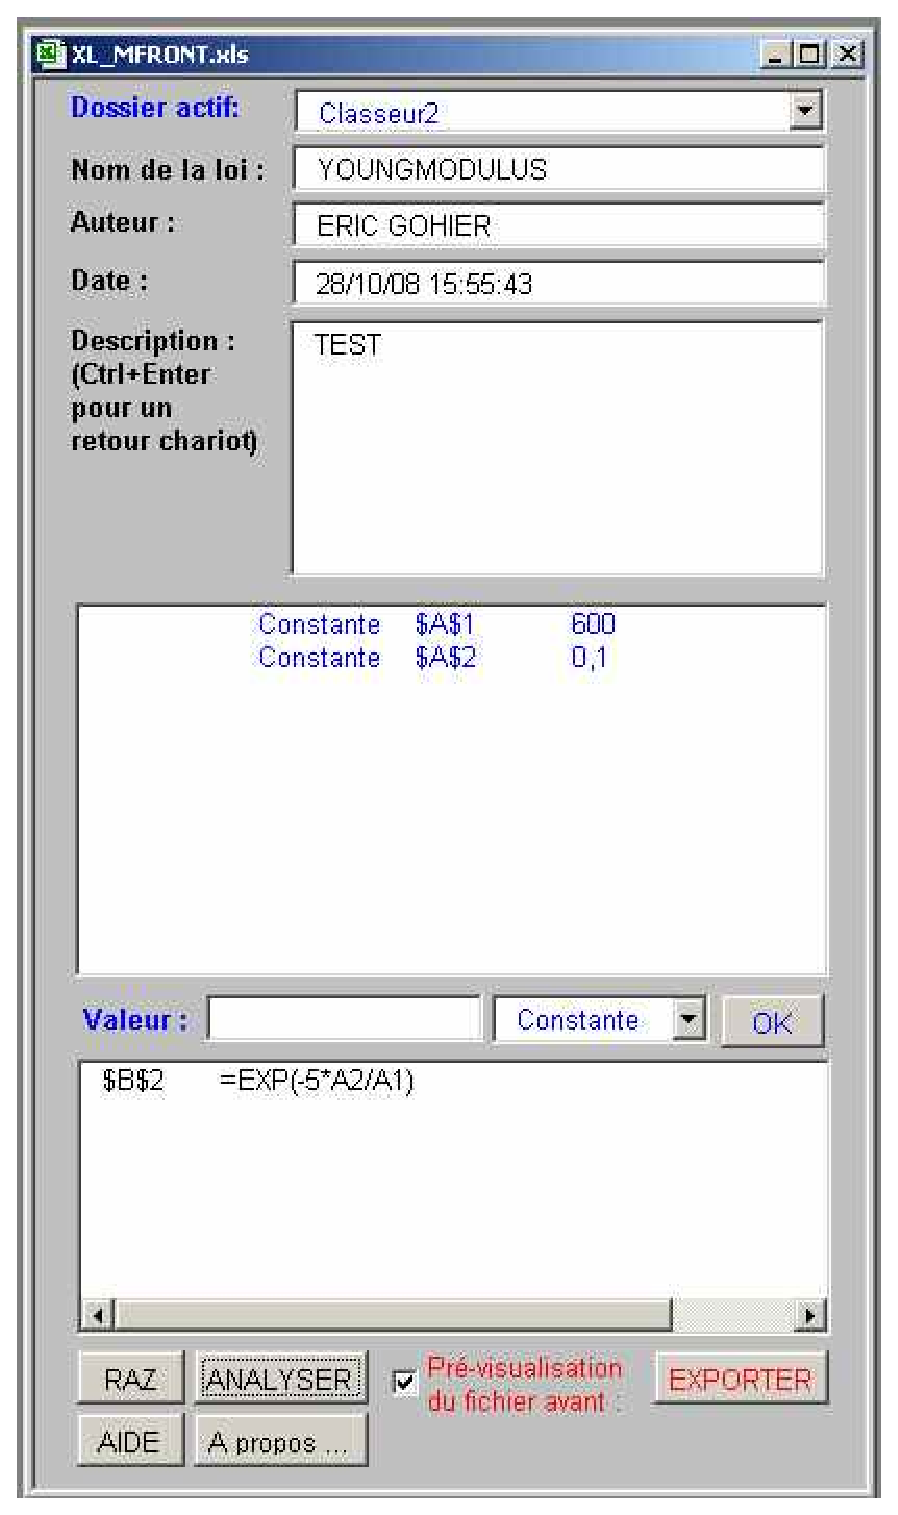
\includegraphics[width=6cm]{Images/mfront.eps}
  \caption{Export d'une formule \excel{} en \mfront{}.}
  \label{fig:exceltomfront}
\end{figure}

\paragraph{De \excel{} à \mfront{}}
De plus il est apparu utile (et relativement facile à mettre en
\oe{}uvre) de pouvoir directement généré des fichiers \mfront{} depuis
des formules \excel{}. Une macro \texttt{Visual Basic} a été écrite
par \nom{É. Gohier} dans ce but. La figure~\ref{fig:exceltomfront}
montre un exemple de son utilisation.

\begin{figure}[htbp]
  \centering
  \code{
    \noindent
\textcolor{blue}{'DEBPROC'}\hspace*{1em}GETEVOL\hspace*{1em}\hspace*{1em}\hspace*{1em}\hspace*{1em}\hspace*{1em}X0\textcolor{magenta}{*}\textcolor{blue}{'FLOTTANT'}\\
\hspace*{1em}\hspace*{1em}\hspace*{1em}\hspace*{1em}\hspace*{1em}\hspace*{1em}\hspace*{1em}\hspace*{1em}\hspace*{1em}\hspace*{1em}\hspace*{1em}\hspace*{1em}\hspace*{1em}\hspace*{1em}\hspace*{1em}\hspace*{1em}\hspace*{1em}\hspace*{1em}\hspace*{1em}\hspace*{1em}\hspace*{1em}\hspace*{1em}X1\textcolor{magenta}{*}\textcolor{blue}{'FLOTTANT'}\\
\hspace*{1em}\hspace*{1em}\hspace*{1em}\hspace*{1em}\hspace*{1em}\hspace*{1em}\hspace*{1em}\hspace*{1em}\hspace*{1em}\hspace*{1em}\hspace*{1em}\hspace*{1em}\hspace*{1em}\hspace*{1em}\hspace*{1em}\hspace*{1em}\hspace*{1em}\hspace*{1em}\hspace*{1em}\hspace*{1em}\hspace*{1em}\hspace*{1em}nx\textcolor{magenta}{*}\textcolor{blue}{'ENTIER'}\\
\hspace*{1em}\hspace*{1em}\hspace*{1em}\hspace*{1em}\hspace*{1em}\hspace*{1em}\hspace*{1em}\hspace*{1em}\hspace*{1em}\hspace*{1em}\hspace*{1em}\hspace*{1em}\hspace*{1em}\hspace*{1em}\hspace*{1em}\hspace*{1em}\hspace*{1em}\hspace*{1em}\hspace*{1em}\hspace*{1em}TLoi\textcolor{magenta}{*}\textcolor{blue}{'TABLE'}\\
\hspace*{1em}\hspace*{1em}\hspace*{1em}\hspace*{1em}\hspace*{1em}\hspace*{1em}\hspace*{1em}\hspace*{1em}\hspace*{1em}\hspace*{1em}\hspace*{1em}\hspace*{1em}\hspace*{1em}\hspace*{1em}\hspace*{1em}\hspace*{1em}\hspace*{1em}\hspace*{1em}\hspace*{1em}\hspace*{1em}vvar\textcolor{magenta}{*}\textcolor{blue}{'MOT'}\\
\hspace*{1em}\hspace*{1em}\hspace*{1em}\hspace*{1em}\hspace*{1em}\hspace*{1em}\hspace*{1em}\hspace*{1em}\hspace*{1em}\hspace*{1em}\hspace*{1em}\hspace*{1em}\hspace*{1em}\hspace*{1em}\hspace*{1em}\hspace*{1em}\hspace*{1em}\hspace*{1em}values\textcolor{magenta}{*}\textcolor{blue}{'TABLE'};\\
\textcolor{blue}{'MESSAGE'}\hspace*{1em}\textcolor{blue}{'---------------------------------'}\hspace*{1em};\\
\textcolor{blue}{'MESSAGE'}\hspace*{1em}\textcolor{blue}{' Début              : '}\hspace*{1em}X0;\\
\textcolor{blue}{'MESSAGE'}\hspace*{1em}\textcolor{blue}{' Fin                : '}\hspace*{1em}X1;\\
\textcolor{blue}{'MESSAGE'}\hspace*{1em}\textcolor{blue}{' Nombre de valeurs  : '}\hspace*{1em}nx;\\
\textcolor{blue}{'MESSAGE'}\hspace*{1em}\textcolor{blue}{' Loi : librairie    : '}\hspace*{1em}TLoi\textcolor{green}{.}\textcolor{blue}{'LIBRAIRIE'};\\
\textcolor{blue}{'MESSAGE'}\hspace*{1em}\textcolor{blue}{' Loi : Modèle       : '}\hspace*{1em}TLoi\textcolor{green}{.}\textcolor{blue}{'MODELE'};\\
vdime=(\textcolor{blue}{'VALEUR'}\hspace*{1em}\textcolor{blue}{'DIME'});\\
velem=(\textcolor{blue}{'VALEUR'}\hspace*{1em}\textcolor{blue}{'ELEM'});\\
\textcolor{blue}{'OPTION'}\hspace*{1em}\textcolor{blue}{'DIME'}\hspace*{1em}\textcolor{green}{1};\\
\textcolor{blue}{'OPTION'}\hspace*{1em}\textcolor{blue}{'ELEM'}\hspace*{1em}SEG2;\\
lx\hspace*{1em}=\hspace*{1em}\textcolor{blue}{'DROIT'}\hspace*{1em}(\textcolor{blue}{'POIN'}\hspace*{1em}X0)\hspace*{1em}(\textcolor{blue}{'POIN'}\hspace*{1em}X1)\hspace*{1em}nx;\\
modv\hspace*{1em}=\hspace*{1em}\textcolor{blue}{'MODELISER'}\hspace*{1em}lx\hspace*{1em}\textcolor{blue}{'THERMIQUE'}\hspace*{1em}\textcolor{blue}{'ISOTROPE'};\\
xx\hspace*{1em}=\hspace*{1em}\textcolor{blue}{'COORDONNEE'}\hspace*{1em}\textcolor{green}{1}\hspace*{1em}lx\hspace*{1em};\\
vpo\hspace*{1em}=\hspace*{1em}\textcolor{blue}{'CHANGER'}\hspace*{1em}xx\hspace*{1em}\textcolor{blue}{'COMP'}\hspace*{1em}vvar;\\
vel\hspace*{1em}=\hspace*{1em}\textcolor{blue}{'CHANGER'}\hspace*{1em}\textcolor{blue}{'CHAM'}\hspace*{1em}vpo\hspace*{1em}modv\hspace*{1em};\\
nb\hspace*{1em}\hspace*{1em}=\hspace*{1em}\textcolor{blue}{'DIME'}\hspace*{1em}(TLoi\textcolor{green}{.}\textcolor{blue}{'VARIABLES'});\\
\textcolor{blue}{'REPETER'}\hspace*{1em}bcl\hspace*{1em}nb;\\
\hspace*{1em}\hspace*{1em}\hspace*{1em}vvari\hspace*{1em}=\hspace*{1em}\textcolor{blue}{'EXTRAIRE'}\hspace*{1em}(Tloi\textcolor{green}{.}\textcolor{blue}{'VARIABLES'})\hspace*{1em}\&bcl;\\
\hspace*{1em}\hspace*{1em}\hspace*{1em}\textcolor{blue}{'SI'}(\textcolor{blue}{'NEG'}\hspace*{1em}vvari\hspace*{1em}vvar);\\
\hspace*{1em}\hspace*{1em}\hspace*{1em}\hspace*{1em}\hspace*{1em}\hspace*{1em}vel\hspace*{1em}=\hspace*{1em}vel\hspace*{1em}\textcolor{blue}{'ET'}\hspace*{1em}(\textcolor{blue}{'MANUEL'}\hspace*{1em}\textcolor{blue}{'CHML'}\hspace*{1em}modv\hspace*{1em}vvari\hspace*{1em}(values\textcolor{green}{.}vvari));\\
\hspace*{1em}\hspace*{1em}\hspace*{1em}\textcolor{blue}{'FINSI'};\\
\textcolor{blue}{'FIN'}\hspace*{1em}bcl;\\
matE\hspace*{1em}=\hspace*{1em}\textcolor{blue}{'MANUEL'}\hspace*{1em}\textcolor{blue}{'CHML'}\hspace*{1em}modv\hspace*{1em}\textcolor{blue}{'Y'}\hspace*{1em}TLoi;\\
Kel\hspace*{1em}=\hspace*{1em}\textcolor{blue}{'VARI'}\hspace*{1em}\textcolor{blue}{'NUAG'}\hspace*{1em}modv\hspace*{1em}matE\hspace*{1em}vel;\\
Kpo\hspace*{1em}=\hspace*{1em}\textcolor{blue}{'CHANGER'}\hspace*{1em}\textcolor{blue}{'CHPO'}\hspace*{1em}Kel\hspace*{1em}modv\hspace*{1em};\\
evabs\hspace*{1em}=\hspace*{1em}\textcolor{blue}{'EVOL'}\hspace*{1em}\textcolor{blue}{'CHPO'}\hspace*{1em}vpo\hspace*{1em}lx\hspace*{1em}vvar;\\
evordo\hspace*{1em}=\hspace*{1em}\textcolor{blue}{'EVOL'}\hspace*{1em}\textcolor{blue}{'CHPO'}\hspace*{1em}Kpo\hspace*{1em}lx\hspace*{1em}\textcolor{blue}{'Y'};\\
labs\hspace*{1em}=\hspace*{1em}\textcolor{blue}{'EXTRAIRE'}\hspace*{1em}evabs\hspace*{1em}\textcolor{blue}{'ORDO'}\hspace*{1em};\\
lordo\hspace*{1em}=\hspace*{1em}\textcolor{blue}{'EXTRAIRE'}\hspace*{1em}evordo\hspace*{1em}\textcolor{blue}{'ORDO'}\hspace*{1em};\\
cou\hspace*{1em}=\hspace*{1em}\textcolor{blue}{'EVOL'}\hspace*{1em}\textcolor{blue}{'MANUEL'}\hspace*{1em}labs\hspace*{1em}vvar\hspace*{1em}lordo\hspace*{1em};\\
cou\hspace*{1em}=\hspace*{1em}cou\hspace*{1em}\hspace*{1em}\textcolor{blue}{'COULEUR'}\hspace*{1em}\textcolor{blue}{'JAUNE'};\\
\textcolor{blue}{'OPTION'}\hspace*{1em}\textcolor{blue}{'DIME'}\hspace*{1em}vdime;\\
\textcolor{blue}{'OPTION'}\hspace*{1em}\textcolor{blue}{'ELEM'}\hspace*{1em}velem;\\
\textcolor{blue}{'FINPROC'}\hspace*{1em}cou\hspace*{1em};

  }
  \caption[Code de la procédure \texttt{GETEVOL}]{Procédure utilisée
    pour tracer les valeurs d'une fonction en fonction d'une de ces
    variables (les autres étant fixées).}
  \label{fig:getEvol}
\end{figure}

\subsection{Interaction avec \castem{}} L'utilisation de
l'interface \castem{} dans les calculs a déjà été décrite par
ailleurs~\cite{helfer07:_utilis}. L'usage a cependant montré qu'il
était très pratique de pouvoir tracer ses fonctions matériaux dans
\castem{}, pour vérification. La procédure \texttt{GETEVOL},
reproduite en figure~\ref{fig:getEvol} a été écrite dans ce but.

\begin{figure}[htbp]
  \centering
  \code{
    \noindent
\textcolor{blue}{'OPTION'}\hspace*{1em}\textcolor{blue}{'DIME'}\hspace*{1em}\textcolor{green}{3};\\
\textcolor{blue}{'OPTION'}\hspace*{1em}\textcolor{blue}{'ELEM'}\hspace*{1em}\textcolor{blue}{'QUA4'};\\
\newline
TLoi\hspace*{1em}=\hspace*{1em}\textcolor{blue}{'TABLE'};\\
TLoi\textcolor{green}{.}\textcolor{blue}{'LIBRAIRIE'}\hspace*{1em}=\hspace*{1em}\textcolor{blue}{'libCastemMaterialLaw.so'};\\
TLoi\textcolor{green}{.}\textcolor{blue}{'MODELE'}\hspace*{1em}\hspace*{1em}\hspace*{1em}\hspace*{1em}=\hspace*{1em}\textcolor{blue}{'SIC\_YOUNGMODULUS\_SNEAD'};\\
TLoi\textcolor{green}{.}\textcolor{blue}{'VARIABLES'}\hspace*{1em}=\hspace*{1em}\textcolor{blue}{'MOTS'}\hspace*{1em}\textcolor{blue}{'T'}\hspace*{1em}\textcolor{blue}{'PORO'};\\
\newline
val\hspace*{1em}=\hspace*{1em}\textcolor{blue}{'TABLE'};\\
val\textcolor{green}{.}\textcolor{blue}{'PORO'}\hspace*{1em}=\hspace*{1em}\textcolor{green}{0.1};\\
\newline
ev\hspace*{1em}=\hspace*{1em}GETEVOL\hspace*{1em}\textcolor{green}{300.}\hspace*{1em}\textcolor{green}{1500.}\hspace*{1em}\textcolor{green}{100}\hspace*{1em}TLoi\hspace*{1em}\textcolor{blue}{'T'}\hspace*{1em}val;\\
\textcolor{blue}{'DESSIN'}\hspace*{1em}ev;

  }
  \caption{Utilisation de la procédure \texttt{GETEVOL}.}
  \label{fig:TestGetEvol}
\end{figure}

Un exemple d'utilisation de cette procédure est donnée en
figure~\ref{fig:TestGetEvol} où est tracé la dépendance du module
d'\nom{Young} du \sic{} en fonction de la température entre $300$ et
$1500$ Kelvins pour une porosité de $0.1$ avec un échantillonnage de
$100$ valeurs. La tableau \texttt{val} contient ici les valeurs de
toutes les variables autre que celle servant au tracé.

\begin{figure}[htbp]
  \centering
  \includegraphics[width=9cm,angle=90]{mfront/GetEvol.eps}
  \caption{Résultat de la procédure \texttt{GETEVOL}.}
  \label{fig:TestGetEvol2}
\end{figure}

La courbe résultante est représentée en figure~\ref{fig:TestGetEvol2}.

\clearpage
\newpage
\section{Tableaux de variables internes, de propriétés matériau et de
  variables externes}

Les versions précédentes de \mfront{} supposait que chaque variable
interne était indépendante et il fallait écrire pour chaque variable les
équations décrivant son évolution. Il n'était pas possible de regrouper
des évolutions dont le {\em formalisme} était similaire.

L'intégration de lois de comportement de plasticité cristalline ou de
lois issus de l'homogénéisation de structures par la méthode
NTFA nous ont montré que cette façon de procéder pouvait devenir mal
commode~: il fallait répéter un grand nombre de fois des équations qui
ne se différenciaient que par leurs coefficients. Le travail
d'intégration présentait alors un caractère répétitif pénible et source
d'erreurs\footnote{Pour illustrer notre propos, nous pouvons donner quelques
  éléments de la méthode NTFA~\cite{blanc:ver}. Le principe de la méthode
  est de décomposer le champ de déformation viscoplastique sur une base
  orthonormée de modes préférentiels de déformation, que l'on identifie
  par des essais élémentaires sur une microstructure
  donnée~\cite{largenton12:_model_mox}. La décomposition s'écrit~:
  \begin{equation}
    \label{eq:decoeps} \epsilonvis(x) = \sum_{k=1}^M \varepsilon^{\mathrm{vis}}_k
    \tenseur{\mu}_k(x)
  \end{equation}
  où~:
  \begin{minipage}[t]{0.9\linewidth}
    \begin{itemize} \item \(M\) le nombre de modes, qui dépend du
      contraste entre les phases, de la nonlinéarité du comportement et
      de la géométrie de milieu~; \item \(\tenseur{\mu}_k\) le k-ième
      mode de déformation plastique (tenseur)~; \item
      \(\varepsilon^{vp}_k\) est la déformation scalaire associée au
      mode \(k\), ces \(M\) déformations sont les {\bf variables
      internes} du modèle.
  \end{itemize}
\end{minipage} \medskip Les modes sont tensoriels, orthonormés,
nonuniformes (dépendants de \(x\)) et à support dans chaque phase. En
viscoélasticité linéaire isotrope incompressible, le système
différentiel régissant l'équilibre global s'écrit en utilisant les
variables réduites scalaires \(e_k\), \(e_k^{\mathrm{vis}}\) et
\(\tau_k\) définies ci-dessous :
\begin{equation}
  \label{eq:modeleeffectif} \displaystyle \left\{
  \begin{array}{rcl}
    \tau_k &=& 2 G_r^e (e_k - e_k^{\mathrm{vis}}) \\
    \dot{e}_k^{\mathrm{vis}} &=& \Frac{1}{2 G_r^{\mathrm{vis}}} \tau_k
    \\
    e_k &=& \tenseur{a}_k : \tenseur{E} + \displaystyle\sum_{l=1}^M
    \Frac{\Big\langle \tenseur{\mu}_k :
      \tenseur{D}^{*}_{\tenseur{\mu}_{l}} \Big\rangle}{\Big\langle
      \tenseur{\mu}_l : \tenseur{\mu}_l \Big\rangle } e_l^{\mathrm{vis}}
    \end{array}
    \right.
  \end{equation}
  où~:
  \begin{minipage}[t]{0.85\linewidth}
    \begin{itemize} \item \(e_k = \langle \tepsilonto : \tenseur{\mu}_k
      \rangle\) \item \(e_k^{\mathrm{vis}} = \langle \epsilonvis :
      \tenseur{\mu}_k \rangle= \langle \tenseur{\mu}_k : \tenseur{\mu}_k
      \rangle \varepsilon^{\mathrm{vis}}_k\) \item \(\tau_k=\langle
      \tsigma : \tenseur{\mu}_k \rangle\) \item \(G_r^e\) est le module
      de cisaillement élastique de la phase \(r\)~; \item
      \(G_r^{\mathrm{vis}}\) est le module de cisaillement
      viscoplastique de la phase \(r\)~; \item \(\tenseur{a}_k = \langle
      \tenseur{\mu}_k :\tenseur{A}\rangle\) le tenseur de localisation
      des déformations réduit~; \item
      \(\tenseur{D}^{*}_{\tenseur{\mu}_{k}}\) est le tenseur
      d'influence associé au mode \(\tenseur{\mu}_k\).
    \end{itemize}
  \end{minipage} \medskip L'évolution de la contrainte macroscopique
  \(\tenseur{\Sigma}\) est donnée par~:
  \[
  \tenseur{\Sigma} = \tenseurq{C} : \tenseur{E} +
  \displaystyle\sum_{k=1}^M \Frac{\Big\langle
    \tenseurq{C}\paren{x}\,\colon\,\tenseur{D}^{*}_{\tenseur{\mu}_{k}}
    \Big\rangle - \Big\langle
    \tenseurq{C}\paren{x}\,\colon\,\tenseur{\mu}_k
    \Big\rangle}{\Big\langle \tenseur{\mu}_k\,\colon\,\tenseur{\mu}_k
    \Big\rangle}e^{\mathrm{vis}}_k
  \]
  où~:
  \begin{minipage}[t]{0.85\linewidth}
    \begin{itemize} \item \(\tenseur{\Sigma}\) est la contrainte
      effective~; \item \(\tenseur{E}\) est la déformation effective~;
      \item \(\tenseurq{C}\paren{x}\) est le tenseur des modules
      élastiques local~; \item \(\tenseurq{C}\) représente le tenseur des
      modules élastiques effectif~;
    \end{itemize}
  \end{minipage}

  Dans le cas de la méthode NTFA, il fallait répéter \(M\) fois, une
  fois pour chaque mode, l'équation~\eqref{eq:modeleeffectif}.
  L'homogénéisation d'une microstructure à \(2\) phases pouvant conduire
  à une trentaine de modes, et l'homogénéisation d'une microstructure à
  \(3\) phases à une cinquantaine de modes, on comprend pourquoi la
  répétition de l'équation~\eqref{eq:modeleeffectif} est
  particulièrement mal venue.}.

Afin de pouvoir regrouper ces équations, nous avons introduit la
possibilité de définir des tableaux de variables internes, de propriétés
matériaux et de variables externes\footnote{Il faut noter que la taille
de ces tableaux, c'est à dire le nombre de variables internes, de
propriétés matériau et/ou de variables externes est fixe \og~en
dur~\fg{} dans le fichier d'entrée. Dans le cas}.

Il est alors possible d'écrire des boucles sur les variables internes
constituant le tableau pour condenser l'écriture des lois.

\begin{figure}
  {\scriptsize
    \hlstd{
@MaterialProperty\ real\ A}\hlsym{{[}}\hlstd{}\hlnum{2}\hlstd{}\hlsym{{]};}\hlstd{\ \ \ \ \ }\hlsym{}\hlstd{}\hlcom{/{*}\ Norton\ coefficient}\hlstd{\ \ \ }\hlcom{{*}/}\hlstd{\hspace*{\fill}\\
@MaterialProperty\ real\ E}\hlsym{{[}}\hlstd{}\hlnum{2}\hlstd{}\hlsym{{]};}\hlstd{\ \ \ \ \ }\hlsym{}\hlstd{}\hlcom{/{*}\ Norton\ exponant}\hlstd{\ \ \ \ \ \ }\hlcom{{*}/}\hlstd{\hspace*{\fill}\\
\ldots\\
\hlstd{
@StateVariable\ real\ p}\hlsym{{[}}\hlstd{}\hlnum{2}\hlstd{}\hlsym{{]};}\hlstd{\ \ \ \ \ \ }\hlsym{}\hlstd{}\hlcom{/{*}\ Equivalent\ viscoplastic\ strain\ {*}/}\hlstd{\hspace*{\fill}\\
@StateVariable\ Stensor\ evp}\hlsym{{[}}\hlstd{}\hlnum{2}\hlstd{}\hlsym{{]};\ }\hlstd{}\hlcom{/{*}\ Viscoplastic\ strain}\hlstd{\ \ \ \ \ \ \ \ \ \ \ \ }\hlcom{{*}/}\hlstd{}\hspace*{\fill}\\
\ldots\\
\hlstd{
@Derivative}\hlsym{\{}\hspace*{\fill}}\\
\hlstd{}\hlstd{\ \ }\hlstd{}\ldots\\
\hlstd{}\hlstd{\ \ }\hlstd{}\hlkwa{for}\hlstd{}\hlsym{(}\hlstd{}\hlkwb{unsigned\ short\ }\hlstd{i}\hlsym{=}\hlstd{}\hlnum{0}\hlstd{}\hlsym{;}\hlstd{i}\hlsym{!=}\hlstd{}\hlnum{2}\hlstd{}\hlsym{;++}\hlstd{i}\hlsym{)\{}\hspace*{\fill}\\
\hlstd{}\hlstd{\ \ \ \ }\hlstd{dp}\hlsym{{[}}\hlstd{i}\hlsym{{]}}\hlstd{\ \ \ \ }\hlsym{=\ }\hlstd{A}\hlsym{{[}}\hlstd{i}\hlsym{{]}{*}}\hlstd{}\hlkwd{pow}\hlstd{}\hlsym{(}\hlstd{sigeq}\hlsym{,}\hlstd{E}\hlsym{{[}}\hlstd{i}\hlsym{{]});}\hspace*{\fill}\\
\hlstd{}\hlstd{\ \ \ \ }\hlstd{devp}\hlsym{{[}}\hlstd{i}\hlsym{{]}}\hlstd{\ \ }\hlsym{=\ }\hlstd{dp}\hlsym{{[}}\hlstd{i}\hlsym{{]}{*}}\hlstd{n}\hlsym{;}\hspace*{\fill}\\
\hlstd{}\hlstd{\ \ \ \ }\hlstd{deel}\hlstd{\ \ \ \ }\hlstd{}\hlsym{{-}=\ }\hlstd{devp}\hlsym{{[}}\hlstd{i}\hlsym{{]};}\hspace*{\fill}\\
\hlstd{}\hlstd{\ \ }\hlstd{}\hlsym{\}}\hspace*{\fill}\\
\hlstd{}\hlsym{\}\ }
  }
  \caption{Exemple de loi de comportement mécanique utilisant des
    tableaux de propriétés matériau et des tableaux de variables
    internes.}
  \label{2norton-rk}
\end{figure}

La figure~\ref{2norton-rk} présente l'exemple d'une loi de comportement
somme de deux écoulements de \textsc{Norton}.

\paragraph{Extension aux intégrations implicites} La possibilité
d'utiliser des tableaux de variables internes est aujourd'hui limitée à
l'intégration par une méthode de \textsc{Runge-Kutta}, son extension à
l'intégration par des méthodes implicites est en cours. La principale
difficulté dans ce cas est de gérer de manière à la fois efficace et
pratique l'accès aux valeurs du jacobien. Cet accès est aujourd'hui
délégué à des variables intermédiaires qui représentent des blocs du
jacobien (voir à ce sujet le paragraphe~\ref{JacobienNumerique}). Ces
variables intermédiaires se comportent comme des tenseurs ou comme des
scalaires (ce qui répond au critère de simplicité d'utilisation), mais
leur utilisation se fait sans coût car il est possible de calculer à la
compilation les décalages mémoire nécessaires pour travailler
directement dans la matrice jacobienne (ce qui répond au critère
d'efficacité). Ceci n'est plus possible avec des tableaux de variables
internes et il est nécessaire donc introduire de nouvelles classes
prenant en compte cette contrainte.

\paragraph{Limitation et possibilité d'amélioration} Pour réduire le
temps de développement de cette fonctionnalité\footnote{Au final, ce
  temps de développement a été de l'ordre de la journée.} et surtout
réduire les sources d'erreurs, nous avons utilisé des classes livrés
avec TFEL (la librairie mathématique sur laquelle se base \mfront{}) qui
propose des vecteurs de taille finie sur lesquelles les opérations
mathématiques usuelles ont été définies. La génération de l'algorithme
de \textsc{Runge-Kutta} est restée inchangée, ce qui est satisfaisant.
Cette solution n'est cependant pas adaptée à un très grand nombre de
variables internes (plus d'une centaine par exemple, ce qui est somme
tout déjà conséquent) car ces classes de vecteurs ont été conçues pour
être optimales pour des petites tailles et leurs utilisations alourdit
le temps de compilation et la taille de la librairie générée. Il s'agit
d'un phénomène connu sous le nom de \og~code bloat~\fg (littéralement,
explosion du code). Des tests, réalisés dans le cadre de la thèse de J.
Souslacroix pour des modèles micromécaniques complexes, ont montré que
ce phénomène était réel et que la tendance à l'augmentation des temps de
compilation et de la taille de la librairie était fortement non
linéaire. Notons enfin que pour des tableaux d'un millier de variables
internes, le temps de compilation pouvait dépasser la minute et que la
taille de la librairie générée pouvait dépasser le mégaoctet, ce qui est
encore relativement raisonnable. Si d'aventure, des lois aussi complexes
devaient être utilisées régulièrement, il serait intéressant de faire
évoluer les classes de vecteurs citées pour limiter ces tentatives
d'optimisation\footnote{Il est d'ailleurs a peu près certain que les
  techniques utilisées n'ont plus d'intérêt pour des vecteurs de cette
  taille.}.

\clearpage
\newpage
\section{Comparaison du jacobien calculé analytiquement par
  l'utilisateur à un jacobien calculé par perturbation numérique}
\label{JacobienNumerique}

L'utilisation de schémas d'intégration implicite, qui transforme un
système différentiel en un système d'équations généralement
non-linéaires, donne souvent des résultats très satisfaisants, tant en
termes de performances que de robustesse\footnote{Ce point peut être
illustré en regardant les résultats obtenus à la section suivante au
tableau~\ref{tab:NR}.}.

Nous associons à chaque variable interne \(X_{i}\) \(\paren{1\leq i\leq
N}\) une équation du système implicite notée
\(f_{X_{i}}\)\footnote{Cette association respecte la nature de la variable
\(X_{i}\)~: si \(X_{i}\) est scalaire, \(f_{X_{i}}\) est scalaire et si
\(X_{i}\) est une variable tensorielle, \(f_{X_{i}}\) est également un
tenseur.}~:
\[
\left\{
\begin{array}{ccc}
f_{X_{1}} & = & 0 \\
\ldots \\
f_{X_{N}} & = & 0 \\
\end{array} \right.
\]

Pour la suite de la note, il est intéressant d'introduire un vecteur
d'inconnus \(\vec{X}\) tel que~:
\[
\vec{X} = \paren{X_{1},\ldots,X_{i},\ldots,X_{N}}
\]
De même, nous pouvons introduire une fonction vectorielle \(\vec{F}\) de
la variable \(\vec{X}\) tel que le système d'équations précédents soit
équivalent à~:
\[
\vec{F}\paren{\vec{X}} = \vec{0}
\]

Pour la résolution du système implicite, un algorithme de
\textsc{Newton-Raphson} est souvent retenu. Cet algorithme est
itératif~: à partir d'une estimation \(\vec{X}_{n-1}\) de la solution
fournit une nouvelle estimation de la solution \(\vec{X}_{n}\) par un
développement limité autour de \(\vec{X}_{n-1}\)~:
\[
\begin{aligned}
F\paren{\vec{X}_{n}} &\approx \vec{F}\paren{\vec{X}_{n-1}}+\left.\deriv{\vec{F}}{\vec{X}}\right|_{\vec{X}=\vec{X_{n-1}}}\,.\,\paren{\vec{X}_{n}-\vec{X}_{n-1}} \\
\end{aligned}
\]

En notant \(J\) la jacobienne \(\deriv{\vec{F}}{\vec{X}}\), et en
imposant que \(\vec{X}_{n}\) est solution du système, nous
obtenons la relation de récurrence suivante\footnote{En pratique,
 l'inverse de la matrice jacobienne n'est jamais calculée et il faut
  comprendre que \(J^{-1}\,.\,\vec{F}\paren{\vec{X}_{n-1}}\) désigne
  la solution \(Y\) du système linéaire~:
  \[
  J\,.\,Y = \vec{F}\paren{\vec{X}_{n-1}}
  \]
  Ce système linéaire est résolu après une factorisation LU de la
  matrice \(J\).}~:
\begin{equation}
  \label{eq:NR}
  \vec{X}_{n}=\vec{X}_{n-1}-J^{-1}\,.\,\vec{F}\paren{\vec{X}_{n-1}}
\end{equation}

L'utilisation de l'algorithme de \textsc{Newton-Raphson} requiert que
l'utilisateur fournisse la matrice jacobienne. En pratique, la matrice
\(J\) est calculée par blocs et prend la forme suivante~:
\[
J = \deriv{\vec{F}}{\vec{X}} =
\begin{pmatrix}
  \deriv{f_{X_{1}}}{X_{1}} & \ldots & \ldots & \ldots & \ldots \\
  \vdots & \vdots & \vdots                   & \vdots & \vdots \\
  \vdots & \vdots & \deriv{f_{X_{i}}}{X_{j}} & \vdots & \vdots \\
  \vdots & \vdots & \vdots                   & \vdots & \vdots \\
  \ldots & \ldots & \ldots & \ldots & \deriv{f_{X_{N}}}{X_{N}} \\
\end{pmatrix}
\]

Or, le calcul de cette matrice est, à juste titre, jugé délicat et une
erreur peut avoir un impact significatif sur les performances ou la
robustesse de l'intégration.

Pour détecter les erreurs dans le calcul du jacobien, nous avons
introduit le mot clé \texttt{@Compare\-To\-Numerical\-Jacobian}. Ce
mot clé déclenche un processus de vérification par comparaison du
jacobien fournit par l'utilisateur à un jacobien évalué numériquement
par perturbations. Cette vérification se fait par étapes~:
\begin{itemize}
  \item la première étape est le calcul d'un jacobien numérique par
  perturbations. Pour gagner en précision, une différence finie centrée
  est utilisée\footnote{En \(1D\), la dérivée numérique d'une fonction
    \(f\) au point \(x\) est évaluée ainsi~:
    \[
    \Frac{f\paren{x+\epsilon}-f\paren{x-\epsilon}}{2\,\epsilon}
    \]
    La perturbation est choisie égale à la valeur du critère d'arrêt de
    l'algorithme implicite.
  }~;
  \item la seconde étape est de comparer les termes du jacobien. La
  comparaison se fait bloc par bloc~: la différence entre la dérivée
  \(\deriv{f_{X_{i}}}{X_{j}}\) calculée par l'utilisateur et son
  approximation numérique \(\Frac{\Delta\,f_{X_{i}}}{\Delta\,X_{j}}\)
  est évaluée ainsi~:
  \[
  \Frac{1}{N_{X_{i}}\,N_{X_{j}}}\norm{\deriv{f_{X_{i}}}{X_{j}}-\Frac{\Delta\,f_{X_{i}}}{\Delta\,X_{j}}}
  \]
  où \(N_{X_{i}}\) est le nombre de composantes de la variables
  \(X_{i}\) et où \(\norm{a}\) est la somme des valeurs absolues des
  composantes de \(a\). Cette différence est comparée à un certain
  critère. Ce critère est par défaut égal au critère de convergence de
  l'algorithme implicite, mais l'utilisateur peut en préciser en autre en
  utilisant le mot clé {\tt @Jacobian\-Comparison\-Criterium}. Si la
  différence est supérieure au critère, un message donnant la valeur de la
  différence, le bloc considéré et son approximation numérique est affiché
  sur la sortie standard.
\end{itemize}

\begin{table}
  \centering
  \begin{tabular}{|c|c|c|}
    \cline{2-3}
    \multicolumn{1}{c|}{} & 
    \begin{minipage}{4cm}
      Nombre de cycles
    \end{minipage} &
    \begin{minipage}{4cm}
      Rapport à la référence
    \end{minipage} \\
    \hline
    Référence             & 4\,776\,120. & 1 \\
    \hline
    \begin{minipage}[p]{4cm}
    Calcul du jacobien numérique et comparaison  
    \end{minipage}
    & 26\,944\,564 & 5,65\\
    \hline
  \end{tabular}
  \label{tab:NR:nJ}
  \caption{Impact du calcul de jacobien numérique et de sa comparaison à
    celui fourni par l'utilisateur.}
\end{table}

\paragraph{Coût du calcul du jacobien numérique et des comparaisons} Le
  coût du calcul du jacobien numérique est souvent important. Nous
  pouvons le constater au tableau~\ref{tab:NR:nJ} où nous avons analysé
  le nombre de cycles processeur à réaliser l'intégration d'une loi de
  \textsc{Norton} lors d'un essai de traction uniaxial\footnote{Cet
  essai est décrit plus en détails au
  paragraphe~\ref{QNR:ComparaisonNumeriques}.}. Pour le cas traité,
le coût de l'intégration est multiplié par \(5,65\). Il faut donc
prendre garde à retirer cette option pour les versions de productions
des lois de comportement.

\clearpage
\newpage
\section{Méthodes de quasi-\textsc{Newton}}

La section précédente a introduit les méthodes implicites et mis en
avant les difficultés associées au calcul du jacobien. Il est alors
intéressant d'introduire d'autres algorithmes de résolution qui ne
nécessitent pas le calcul du jacobien ou, du moins, permettent de
n'utiliser qu'une approximation de celui-ci.

De manière général, nous pouvons modifier l'algorithme~\eqref{eq:NR} en
substituant à la matrice jacobienne une matrice
\(\underset{\sim}{J}\) bien choisie~:
\begin{equation}
  \label{eq:QNR}
  \vec{X}_{n}=\vec{X}_{n-1}-\underset{\sim}{J}^{-1}\,.\,\vec{F}\paren{\vec{X}_{n-1}}
\end{equation}

Une première solution est d'utiliser une matrice \(\underset{\sim}{J}\)
constante, mais cela est souvent insuffisant en cas de forte non
linéarité. Différentes solutions sont maintenant proposées. Elles seront
comparées, en termes de coût d'intégration, au
paragraphe~\ref{QNR:ComparaisonNumeriques}.

\subsection{Calcul numérique du jacobien}

Nous pouvons approximer le jacobien par différentiation numérique. Cette
méthode présente deux variantes~:
\begin{itemize}
  \item l'ordre de différentiation peut être d'ordre \(1\) ou d'ordre
  \(2\)~;
  \item l'approximation numérique peut être réactualisée à différentes
  fréquences.
\end{itemize}

Un jacobien correctement évalué (ordre \(2\) et réactualisé souvent
conduira à une meilleure convergence de l'algorithme, mais peut avoir un
coût numérique important qui annule le bénéfice de cette meilleure
convergence (voir au paragraphe~\ref{QNR:ComparaisonNumeriques} les
tableaux~\ref{tab:QNR:1} et~\ref{tab:QNR:2}).

\subsection{Les algorithmes de \textsc{Broyden}}

Nous décrivons dans ce paragraphe deux algorithmes dû à \textsc{Broyden}.

\subsubsection{Premier algorithme de \textsc{Broyden}}

Un des algorithmes les plus utilisés est celui de \textsc{Broyden} qui
met à jour au cours des itérations une approximation
\(\underset{\sim}{J}_{n}\) de la matrice jacobienne à partir de son
expression \(\underset{\sim}{J}_{n-1}\) à l'itération
précédente~:
\begin{equation}
  \label{eq:Broyden}
  \underset{\sim}{J}_{n} = \underset{\sim}{J}_{n-1}+\Frac{\Delta\,\vec{F}_{n}-\underset{\sim}{J}_{n-1}\,.\,\Delta\vec{X}_{n}}{\norm{\Delta\,\vec{X}_{n}}^{2}}\otimes\Delta\vec{X}_{n}
\end{equation}
où~:
\begin{minipage}[t]{0.8\linewidth}
  \begin{itemize}
    \item \(\Delta\,\vec{X}_{n}=\vec{X}_{n}-\vec{X}_{n-1}\)~;
    \item \(\Delta\,\vec{F}_{n}=\vec{F}\paren{\vec{X}_{n}}-\vec{F}\paren{\vec{X}_{n-1}}\)~;
    \item \(\vec{v}_{1}\,\otimes\,\vec{v}_{2}\) est le produit tensoriel
    de deux vecteurs~;
    \item \(\norm{\vec{v}}\) est la norme euclidienne du vecteur
    \(\vec{v}\).
  \end{itemize}
\end{minipage}

\paragraph{Calcul exact de certains blocs}
Il est intéressant de remarquer qu'il est toujours possible de modifier
la matrice jacobienne par blocs~: si certains termes sont connus et/ou
facile à calculer, il peut être intéressant de les injecter dans la
matrice jacobienne en écrasant les modifications fournies par
l'algorithme de \textsc{Broyden}.

\paragraph{Initialisation du jacobien} Il est nécessaire de fournir une
estimation initiale \(\underset{\sim}{J}_{0}\) du jacobien. Deux
choix ont été regardé dans cette note~:
\begin{itemize}
  \item \(\underset{\sim}{J}_{0}\) est choisi égal à l'identité~;
  \item \(\underset{\sim}{J}_{0}\) est calculé par perturbations du
  système initial.
\end{itemize}

\subsubsection{Second algorithme de \textsc{Broyden}}

Une variante de l'algorithme de \textsc{Broyden} met à jour une
approximation \(\underset{\sim}{J}_{n}^{-1}\) de l'inverse de la matrice
jacobienne par la relation suivante~:
\begin{equation}
  \label{eq:Broyden2}
  \underset{\sim}{J}_{n}^{-1} =
  \underset{\sim}{J}_{n-1}^{-1}+\Frac{\Delta\,\vec{X}_{n}-\underset{\sim}{J}_{n-1}^{-1}\,.\,\Delta\,\vec{F}_{n}}{\Delta\,\vec{X}_{n}\,\mid\,\underset{\sim}{J}_{n-1}^{-1}\,.\,\Delta\,\vec{F}_{n}}\,\otimes\,\paren{\Delta\,\vec{X}_{n}\,\mid\,\underset{\sim}{J}_{n-1}^{-1}}
\end{equation}
  
Cette variante est disponible dans \mfront{} sous le nom de
\texttt{Broyden2}.

\clearpage
\newpage
\section{Conclusions}

Ca se développe bien (DMN+DER+cyrano) !

\subsection{Perspectives de développement}

\begin{itemize}
  \item passage en déformations finies~;
  \item possibilité d'utiliser des tableaux de variables internes dans
  les algorithmes implicites~;
  \item améliorer la robustesse des intégrations implicites.
  Perspectives de travail avec les expert d'eDF.
\end{itemize}

\clearpage
\newpage
\bibliographystyle{fr-insa}
\bibliography{Bibliographie} 

\appendix

\clearpage
\newpage
\section{Amélioration de la robustesse des algorithmes de résolutions
  implicites}

Les méthodes de résolution des systèmes implicites nécessitent de
choisir une estimation de la solution \(\vec{X}_{0}\) pour initier la
recherche. Par défaut, \mfront{} utilisera le vecteur nul comme
estimation initiale, mais l'utilisateur peut en spécifier une autre par
la directive \texttt{@Predictor}.

La convergence des algorithmes de résolutions implicites n'est garantie
que si l'estimation initiale \(\vec{X}_{0}\) est suffisamment proche de
la solution recherchée. Loin de la solution, l'algorithme peut
éventuellement converger mais les premières itérations tendent
généralement vers la solution assez lentement (phase de recherche)~: il
est classique d'observer une convergence linéaire lors de la phase de
recherche et une transition vers un ordre de convergence plus élevé
proche de la solution.

Pour les lois de comportement fortement non linéaires, il est difficile
de proposer une estimation \(\vec{X}_{0}\) garantissant la convergence,
il peut donc être intéressant d'améliorer la robustesse des algorithmes.

\begin{table}
  \centering
  \begin{tabular}{|c|c|}
    \hline
    Méthode & Expression de \(\vec{s}_{n}\) \\
    \hline
    \hline
    Algorithme de \textsc{Newton-Raphson}
    & \(-J^{-1}\,.\,\vec{F}\paren{\vec{X}_{n-1}}\) \\
    \hline
    \begin{minipage}{7cm}
      Algorithme de \textsc{Newton-Raphson} et dérivation numérique
    \end{minipage} &
    \(-\underset{\sim}{J}^{-1}\,.\,\vec{F}\paren{\vec{X}_{n-1}}\) \\
    \hline
    Premier algorithme de \textsc{Broyden} &
    \begin{minipage}{5cm}
      \(-\underset{\sim}{J}_{n-1}^{-1}\,.\,\vec{F}\paren{\vec{X}_{n-1}}\)
      où \(\underset{\sim}{J}_{n}\) est donné par
      l'équation~\eqref{eq:Broyden}
    \end{minipage} \\
    \hline
    Second algorithme de \textsc{Broyden} &
    \begin{minipage}{5cm}
      \(-\underset{\sim}{J}_{n-1}^{-1}\,.\,\vec{F}\paren{\vec{X}_{n-1}}\)
      où \(\underset{\sim}{J}_{n}^{-1}\) est donné par\(\vec{X}_{0}\)
      l'équation~\eqref{eq:Broyden2}
    \end{minipage} \\
    \hline
  \end{tabular}
  \label{tab:sn}
\end{table}

L'ensemble des algorithmes présentés jusqu'ici prennent la forme~:
\[
\vec{X}_{n}=\vec{X}_{n-1}+\vec{s}^{N}_{n}
\]
L'expression du pas \(s^{N}_{n}\) pour les différentes algorithmes
présentés est donnée au tableau~\ref{tab:sn}. D'après la discussion
précédente, ce pas \(s^{N}_{n}\) est optimal proche de la solution
finale.

Il est intéressant de trouver une autre estimation de la solution, moins
performante près de la solution mais plus robuste. Les méthodes
précédentes donnant une approximation du jacobien, il peut être
intéressant de substituer à la fonction \(F\) son application tangente
et de choisir cette nouvelle estimation comme la solution du problème de
minimisation suivant~:
\[
\min_{\vec{s}^{G}\,\in\,\mathcal{R}^{N}}\,\norm{\vec{F}\paren{\vec{X}_{n-1}}+J\paren{\vec{X}_{n-1}}\,.\,\vec{s}^{G}}
\]

La solution de ce problème est donnée par\footnote{Pour le prouver,
  nous pouvons écrire que~:
  \[
  \begin{array}{rcl}
    \norm{\vec{F}\paren{\vec{X}_{n-1}}+J\paren{\vec{X}_{n-1}}\,.\,\vec{s}^{G}}^{2}
    &=& {F}\paren{\vec{X}_{n-1}}\,.\,{F}\paren{\vec{X}_{n-1}}+2\,\vec{F}\paren{\vec{X}_{n-1}}\,\mid\,J\paren{\vec{X}_{n-1}}\,.\,\vec{s}^{G} \\
    &&+\paren{J\paren{\vec{X}_{n-1}}\,.\,\vec{s}^{G}}\,\mid\,\paren{J\paren{\vec{X}_{n-1}}\,.\,\vec{s}^{G}}
  \end{array}
  \]
  Le gradient de cette expression est égal à~:
  \[
  2\,\mbox{}^{t}J\paren{\vec{X}_{n-1}}\vec{F}\paren{\vec{X}_{n-1}}+\mbox{}^{t}J\paren{\vec{X}_{n-1}}\,J\paren{\vec{X}_{n-1}}\,.\vec{s}^{G}
  \]
}~:
\[
\mbox{}^{t}J\paren{\vec{X}_{n-1}}\,J\paren{\vec{X}_{n-1}}\,.\vec{s}^{G}=-\,\mbox{}^{t}J\paren{\vec{X}_{n-1}}\,.\,\vec{F}\paren{\vec{X}_{n-1}}
\]
Ce pas est intéressant loin de la solution.

Les pas \(\vec{s}^{N}_{n}\) et \(\vec{s}_{n}^{G}\) sont combinés ainsi~:
\[
\vec{s} = a_{n} \,\vec{s}^{G}_{n} + \paren{1-a_{n}}\,\vec{s}_{n}^{N}
\]

\clearpage
\newpage
\section{Comparaisons numériques de différents algorithmes de résolution}
\label{QNR:ComparaisonNumeriques}

\paragraph{Loi utilisée pour la comparaison}

%\paragraph{}

Nous comparons ici les méthodes 

\begin{figure}[htbp]
  \centering
  \includegraphics[height=0.8\linewidth,angle=-90]{Images/CompSeq.eps}
  \caption{Contraintes équivalentes obtenues respectivement par une
    résolution par un algorithme de \textsc{Newton-Raphson} ou par un
    algorithme de \textsc{Broyden}.}
  \label{fig:CompVMis}
\end{figure}


\begin{table}
  \centering
  \begin{tabular}[htbp]{|c|c|c|}
    \hline
    Variante & Nombre de cycles &
    \begin{minipage}{4cm}
      \begin{center}
        Ratio par rapport à \\
        l'algorithme de \textsc{Newton}
      \end{center}
    \end{minipage} \\
    \hline
    \hline
    \(J\) exact & \(4\,707\,335\)  & 1\\
    \hline
    \begin{minipage}[p]{5cm}
      \begin{center}
        \(J\) égal à l'identité
      \end{center}
    \end{minipage}
    & pas de convergence  & \\
    \hline
    \begin{minipage}[p]{5cm}
      \begin{center}
        \(\deriv{f_{\tepsilonel}}{\Delta\,\tepsilonel}\) et
        \(\deriv{f_{p}}{\Delta\,p}\) exacts
      \end{center}
    \end{minipage} &
    pas de convergence & \\
    \hline
    \begin{minipage}[p]{5cm}
      \begin{center}
        \(\deriv{f_{p}}{\Delta\,\tepsilonel}\) et
        \(\deriv{f_{p}}{\Delta\,p}\) exacts, et
        \(\deriv{f_{\tepsilonel}}{\Delta\,\tepsilonel}\) égal à
        l'identité
      \end{center}
    \end{minipage} &
    pas de convergence & \\
    \hline
    \begin{minipage}[p]{5cm}
      \begin{center}
        \(\deriv{f_{\tepsilonel}}{\Delta\,p}\) et
        \(\deriv{f_{p}}{\Delta\,p}\) exacts, et
        \(\deriv{f_{\tepsilonel}}{\Delta\,\tepsilonel}\) égal à
        l'identité
      \end{center}
    \end{minipage} &
    \(152\,721\,841\) & \(32.44\)\\
    \hline
  \end{tabular}
  \label{tab:NR}
  \caption{Temps calculs obtenus avec l'algorithme de
    \textsc{Newton-Raphson}.}
\end{table}

\begin{table}
  \centering
  \begin{tabular}[htbp]{|c|c|c|}
    \hline
    Variante & Nombre de cycles &
    \begin{minipage}{4cm}
      \begin{center}
        Ratio par rapport à \\
        l'algorithme de \textsc{Newton}
      \end{center}
    \end{minipage} \\
    \hline
    \hline
    \(\underset{\sim}{J}\) réactualisé à chaque itération          & \(9\,900\,064\) & \(2,10\) \\
    \hline
    \(\underset{\sim}{J}\) réactualisé toutes les \(2\) itérations & \(8\,674\,464\) & \(1,84\) \\
    \hline
    \(\underset{\sim}{J}\) réactualisé toutes les \(3\) itérations & \(9\,159\,968\) & \(1,94\) \\
    \hline
  \end{tabular}
  \label{tab:QNR:1}
  \caption{Temps calculs obtenus avec l'algorithme de
    quasi-\textsc{Newton} et un calcul numérique du jacobien par une
    différence finie (approximation d'ordre \(1\)).}
\end{table}

\begin{table}
  \centering
  \begin{tabular}[htbp]{|c|c|c|}
    \hline
    Variante & Nombre de cycles &
    \begin{minipage}{4cm}
      \begin{center}
        Ratio par rapport à \\
        l'algorithme de \textsc{Newton}
      \end{center}
    \end{minipage} \\
    \hline
    \hline
    \(\underset{\sim}{J}\) réactualisé à chaque itération & \(14\,916\,316\)  & \(3,16\)        \\
    \hline
    \(\underset{\sim}{J}\) réactualisé toutes les \(2\) itérations & \(11\,773\,880\) & \(2,5\) \\
    \hline
    \(\underset{\sim}{J}\) réactualisé toutes les \(3\) itérations & \(13\,330\,216\) & \(2,83\) \\
    \hline
  \end{tabular}
  \label{tab:QNR:2}
  \caption{Temps calculs obtenus avec l'algorithme de
    quasi-\textsc{Newton} et un calcul numérique du jacobien par une
    différence finie centrée (approximation d'ordre \(2\)).}
\end{table}


\begin{table}
  \centering
  \begin{tabular}[htbp]{|c|c|c|}
    \hline
    Variante & Nombre de cycles &
    \begin{minipage}{5cm}
      \begin{center}
        Ratio par rapport à \\
        l'algorithme de \textsc{Newton}
      \end{center}
    \end{minipage} \\
    \hline
    \hline
    Défaut    & \(20\,197\,423\) & \(4,29\)\\
    \hline
    \(J\) exact & \(6\,120\,862\) & \(1,3\)\\
    \hline
    \(\deriv{f_{\tepsilonel}}{\Delta\,\tepsilonel}\) exact &
    \(36\,821\,766\) & \(7,82\)\\
    \hline
    \(\deriv{f_{p}}{\Delta\,p}\) exact &
    \(33\,826\,368\) & \(7,186\)\\
    \hline
    \(\deriv{f_{p}}{\Delta\,\tepsilonel}\) exact &
    \(19\,577\,698\) & \(4,15\)\\
    \hline
    \(\deriv{f_{\tepsilonel}}{\Delta\,p}\) exact &
    \(12\,132\,956\) & \(2,58\)\\
    \hline
    \(\deriv{f_{\tepsilonel}}{\Delta\,p}\) et \(\deriv{f_{p}}{\Delta\,\tepsilonel}\) exacts &
    \(4\,686\,228\) & \(0,995\) \\
    \hline
  \end{tabular}
  \label{tab:Broyden:1}
  \caption{Temps calculs obtenus avec le premier algorithme de
    \textsc{Broyden} et jacobien initial égal à l'identité.}
\end{table}

\begin{table}
  \centering
  \begin{tabular}[htbp]{|c|c|c|}
    \hline
    Variante & Nombre de cycles &
    \begin{minipage}{5cm}
      \begin{center}
        Ratio par rapport à \\
        l'algorithme de \textsc{Newton}
      \end{center}
    \end{minipage} \\
    \hline
    \hline
    Défaut & \(9\,535\,347\) & \(2,02\) \\
    \hline
    \(\deriv{f_{\tepsilonel}}{\Delta\,p}\) et \(\deriv{f_{p}}{\Delta\,\tepsilonel}\) exacts &
    \(8\,178\,547\) & \(1,73\) \\
    \hline
  \end{tabular}
  \label{tab:Broyden:2}
  \caption{Temps calculs obtenus avec le premier algorithme de
    \textsc{Broyden} et jacobien initial approximé numériquement.}
\end{table}

\begin{table}
  \centering
  \begin{tabular}[htbp]{|c|c|c|}
    \hline
    Variante & Nombre de cycles &
    \begin{minipage}{5cm}
      \begin{center}
        Ratio par rapport à \\
        l'algorithme de \textsc{Newton}
      \end{center}
    \end{minipage} \\
    \hline
    \hline
    Défaut    & \(19\,530\,077\) & \(4,15\)\\
    \hline
  \end{tabular}
  \label{tab:Broyden2}
  \caption{Temps calculs obtenus avec le second algorithme de
    \textsc{Broyden} et jacobien initial égal à l'identité.}
\end{table}

\paragraph{Comparaison des algorithmes de \textsc{Broyden}} En comparant
  les résultats donnés par les tableaux~\ref{tab:Broyden:1},
  \ref{tab:Broyden:2} et~\ref{tab:Broyden2}, nous pouvons constater que le s

\end{document}